\documentclass[11pt,a4paper]{article}
\usepackage[margin=18mm,headheight=14pt]{geometry}
\usepackage[T1]{fontenc}
\usepackage{needspace}
\usepackage{lmodern,microtype,booktabs,tabularx,array,xcolor,hyperref,fancyhdr,amsmath,graphicx}
\graphicspath{{figures/}}
\usepackage{tikz}
\usetikzlibrary{positioning,arrows.meta,calc}
\hypersetup{colorlinks=true,urlcolor=blue!50!black,linkcolor=black}
\setlength{\parindent}{0pt}
\setlength{\parskip}{4pt}
\setlength{\emergencystretch}{3em}
\newcommand{\rp}[1]{\path{#1}}
\newcommand{\subhead}[1]{\Needspace{5\baselineskip}\vspace{0.5em}\noindent{\bfseries #1}\par\vspace{-0.1em}}
\pagestyle{fancy}\fancyhf{}\lhead{\small ARIADNE / AGENTIC VISION}\rhead{\small OpenCV AI Competition 2026}\cfoot{\thepage}
\begin{document}
\begin{center}
{\Large\bfseries From Visual Evidence to Mission Decisions}\\[3pt]
{\small Ariadne | Agentic Vision award evidence | Technical companion to the main report}
\end{center}
\vspace{-0.6em}

\subhead{An agent acts on a changing map}
Ariadne closes a perception--decision--action loop for multiple camera-equipped agents exploring an uncertain interior. OpenCV 5 extracts tracks, stereo depth and geometric correspondences; the stereo-inertial estimator turns these into keyframe poses and mapped surfaces. As observations accumulate, a deterministic planner refreshes feasible viewpoints, map-support needs, traversability and return constraints. Amazon Bedrock Nova 2 Lite uses MCP tools to inspect this bounded situation and choose tasks. A validated command moves an agent, whose next camera observations change the map and its subsequent choices.

\begin{center}
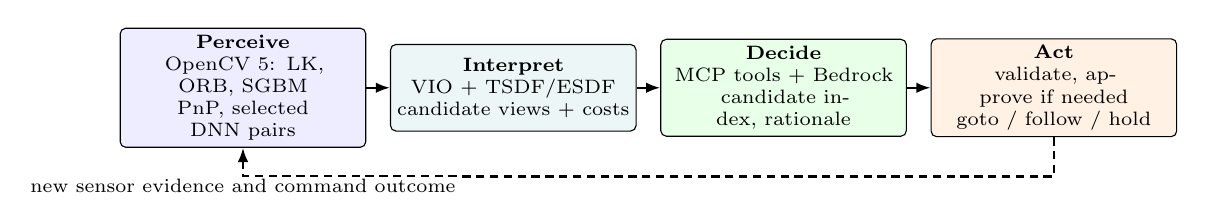
\begin{tikzpicture}[>=Latex,node distance=3mm and 3mm,
 b/.style={draw,rounded corners=2pt,align=center,minimum height=11mm,text width=29.5mm,inner sep=2.4pt,font=\scriptsize},
 a/.style={-{Latex[length=1.8mm]},thick}]
 \node[b,fill=blue!7] (eye) {\textbf{Perceive}\\OpenCV 5: LK, ORB, SGBM\\PnP, selected DNN pairs};
 \node[b,fill=teal!7,right=of eye] (world) {\textbf{Interpret}\\VIO + TSDF/ESDF\\candidate views + costs};
 \node[b,fill=green!9,right=of world] (choice) {\textbf{Decide}\\MCP tools + Bedrock\\candidate index, rationale};
 \node[b,fill=orange!11,right=of choice] (move) {\textbf{Act}\\validate, approve if needed\\goto / follow / hold};
 \draw[a] (eye)--(world);\draw[a] (world)--(choice);\draw[a] (choice)--(move);
 \draw[a,densely dashed] (move.south) -- ++(0,-5mm) -| node[below,pos=.52,font=\scriptsize,fill=white,inner sep=1pt]{new sensor evidence and command outcome} (eye.south);
\end{tikzpicture}
\end{center}

\subhead{The geometric contract behind a decision}
The frame-rate path propagates landmarks through pyramidal LK (\texttt{cv::calcOpticalFlowPyrLK}, $21$-pixel window, four levels), forward/backward rejection at $0.5$\,px, and seeded USAC epipolar checks at $1$\,px. On the $1280\times720$ stereo rig, FAST/ORB replenishes up to $1{,}500$ keypoints over a $12\times7$ grid, targeting $500$ active tracks at $25$\,px spacing. Keyframes are triangulated from a left--right LK match on the rectified row and cross-checked against StereoSGBM depth; a ten-keyframe stereo-inertial optimizer (Schur-complement Levenberg--Marquardt on OpenCV's \texttt{cv::detail::LevMarqBase}, Forster IMU preintegration) estimates pose, velocity, biases and selected covariances, and keyframes leaving the window become pose-graph edges with intra-agent loop closure. At recognition events, EigenPlaces proposes overlapping places, while OpenCV ALIKED--LightGlue and PnP verify selected pairs before robust graph merging. This geometry changes the state exposed to the mission planner and the model's tools.

A view sampler turns frontiers, uncertain cells, inter-agent revisits, alias hypotheses and weakly supported egress segments into candidate observations. It samples radii of $1.0$, $1.5$ and $2.0$\,m over sixteen azimuths; collision and line-of-sight checks gate feasibility. A $64$-ray coarse pass and $256$-ray detailed pass value expected coverage, entropy, responder-route support, graph connectivity and alias resolution, with path, bandwidth and risk costs deducted. CBBA exchanges winner/bid state to allocate stable tasks; the deterministic planner also maintains responder-sized routes through known traversable space. The LLM receives candidate indices, map renderings, uncertainty, fleet state and route summaries. It chooses among available tasks without producing arbitrary coordinates or overriding geometric clearance.

\subhead{Orchestration, transport, and the operator}
The live path connects Gazebo Harmonic and ROS 2 Jazzy through a composed \texttt{ros\_gz\_bridge} and \texttt{RuntimeLink}. Typed observations cross a length-prefixed CDR socket into the ROS-independent \texttt{ariadne\_live} estimator and planner. The runtime consumes ordered sensor events, records them as \rp{inputs.mcap}, and advances replanning at deterministic simulation-time barriers. The model receives one joint chooser request per replan through Bedrock Converse; MCP exposes map, image, uncertainty, route and task queries. The response contains candidate indices and rationales. The same validation path checks candidate membership, reachability, risk, and uniqueness before issuing \texttt{goto}, \texttt{follow} or \texttt{hold} to a collision-checked kinematic mover. Its acknowledgements, refusals and executed segments feed the next planning state.

The hosted operator frontend at \url{https://www.ariadne.cynicpixel.xyz/} presents camera feature overlays, trajectories, uncertainty, task assignments, link traffic and responder routes. It supports replay, agent controls and collaboration actions including link interruption, restoration and false-edge injection. In the three-agent demo, feature overlays displayed $491$, $371$ and $298$ image points in an inspected frame. Gaussian submaps provide a companion spatial view through Spark/WebGL: the live receiver ingested $71$ keyframes with zero tee drops and exported four submaps containing $259{,}994$ seeded Gaussians. The reconstructed scene and labelled ground-truth view remain visually distinguishable.

\subhead{Observed decisions and action outcomes}
\begin{center}
\footnotesize
\begin{tabularx}{\linewidth}{@{}p{34mm}p{75mm}X@{}}
\toprule
\textbf{Run / intervention} & \textbf{Recorded outcome} & \textbf{What it establishes}\\
\midrule
\textbf{Final integrated stack} (AWS, 2 agents, 200\,s) & 40 joint replans, \textbf{80 Nova~2~Lite decisions, 80/80 validated}, no fallback, no answer timeout; 80 commands (70 \texttt{goto}, 8 \texttt{follow}, 2 \texttt{turn}); mover accepted 79 of 82 command states and refused 3 at the 0.20\,m ESDF collision envelope; 4{,}001 frames and 335/342 keyframes per agent; replay PASS; GPU splat from 677 keyframes. Source: \texttt{c143db14} plus a recorded working-tree diff (live wiring of the full VIO configuration, \rp{source_status.txt}). & Full perception (VIO with IMU and loop closure) $\rightarrow$ map $\rightarrow$ MCP/Bedrock $\rightarrow$ validated command $\rightarrow$ mover, end to end, reproducible.\\
Live two-agent loop & 45\,s local run, 13 accepted commands, zero refusals; estimator replay identical twice. & Perceive--choose--move--observe behavior with the real mover interface.\\
First Bedrock loop & 90\,s, 18 joint replans, 36/36 Nova~2~Lite assignments, no fallbacks; 15/15 replay checks. & Sustained model-in-the-loop operation.\\
Three-agent coordination & 20\,s, six coordinated assignments; three initial no-consensus and three no-assignment events; two replays passed. & Consensus, no-duplicate assignment and live communication visibility.\\
Matched 90\,s chooser & 18 joint replans and 36 per-agent decisions per arm. Bedrock differed from classical agent 0 on $6/18$ replans; rank-zero selection $31/36$ vs $26/36$. & A controlled difference at the decision boundary, with one shared source revision and scene/seed.\\
Command outcomes & Each 90\,s arm issued 36 commands: 34 accepted, none refused, two without a terminal reply before run end. & Execution acknowledgements and outcome logging.\\
Matched 500\,s chooser & 100 joint replans, 200 commands and 10,001 frames per agent in each arm; two independent replays per arm passed. & Sustained bounded orchestration and repeatable recorded behavior.\\
Allocation oracle & CBBA matched centralized greedy on 40/40 replans; mean $0.994$ of exact optimum on 12 linked cases; 11.8\,kB sparse traffic vs 123.4\,kB dense. & Task-consensus correctness and measured message economy in its tested replay.\\
\bottomrule
\end{tabularx}
\end{center}

\begin{center}
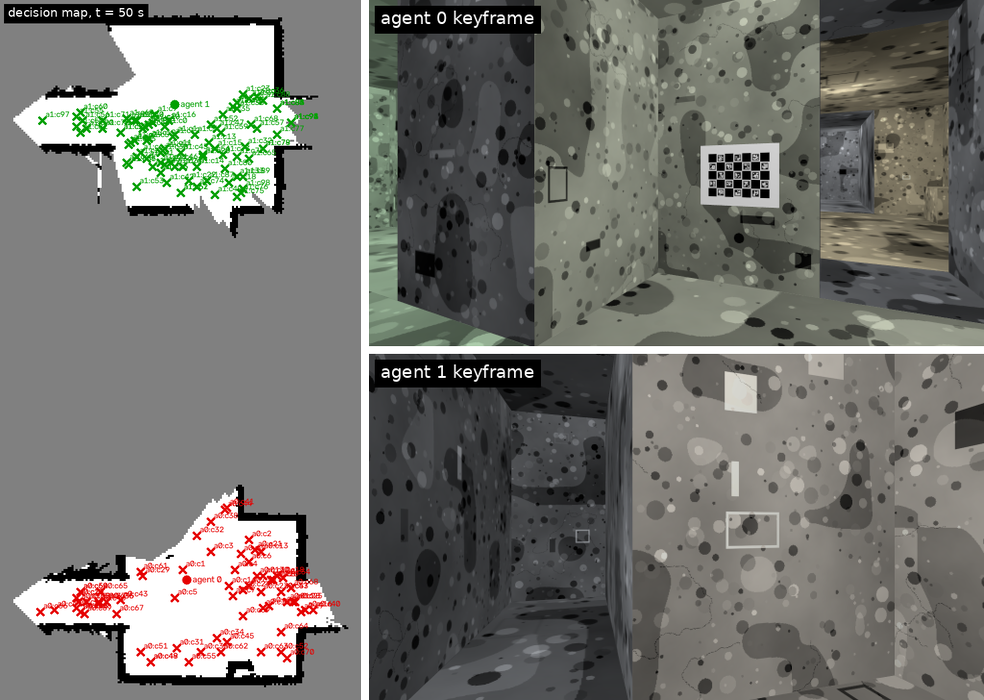
\includegraphics[width=0.92\linewidth]{fig_decision.png}\\[-0.2em]
{\footnotesize Final-stack run, decision at $t=50$\,s: the OpenCV-rendered map the model receives through \texttt{observe\_image} (each agent's candidate goals marked) and both agents' keyframes at that instant.}
\end{center}

\textbf{Final-stack decision statistics} (\rp{trace.jsonl}, 80 agent records). Tool use per joint decision: \texttt{list\_candidates}, \texttt{query\_route} and \texttt{assign} 40 each, \texttt{observe\_map} and \texttt{query\_uncertainty} 74 each, \texttt{observe\_image} 31; 196 Bedrock calls in total. Orchestration latency median $3.43$\,s, p90 $9.40$\,s, maximum $13.22$\,s. The model chose the planner's rank-0 candidate in 73 of 80 records and departed from the classical choice in 6. Every record offered at least one candidate flagged \texttt{needs\_approval}; the model selected one in \textbf{0 of 80}.

The 90-second Bedrock arm spent a median $5.8$\,s per model/tool orchestration cycle (p90 $7.45$\,s; maximum $9.03$\,s), excluding C++ motion and planning. Its trace recorded $2{,}936{,}424$ cumulative input tokens over $118$ calls; repeated tool-context submission contributes to that count. The chooser comparisons demonstrate distinct, replayable behavior. Mission-quality superiority would require paired ground-truth coverage, completion and egress scores, which were outside these matched arms.

\subhead{Causal trace and failure handling}
The observable chain is \emph{OpenCV frame features and stereo geometry $\rightarrow$ updated pose/depth and task candidates $\rightarrow$ MCP map/candidate query $\rightarrow$ Bedrock-selected candidate $\rightarrow$ mover command and acknowledgement $\rightarrow$ subsequent frames}. The repository retains camera overlays, estimator state, candidate lists, model/tool traces, \rp{telemetry.jsonl}, \rp{mover_agent_<k>.jsonl}, and live-to-replay digests. For judge inspection, a single recorded joint replan can be opened at its timestamp and followed through those artifacts, including the six agent-0 decisions where Bedrock selected a different task from the matched classical arm. This is a traceable perception-to-action dependency; the experiments do not isolate an individual OpenCV primitive as the cause of the chooser-arm difference.

A concrete chain from the final-stack run (agent~0). Stereo keyframes integrated into the TSDF raised the mapped free cells $0\rightarrow1{,}986\rightarrow3{,}205\rightarrow6{,}628\rightarrow8{,}537$ between $t=10$ and $30$\,s, and the candidate set grew with them ($16\rightarrow40\rightarrow48\rightarrow63\rightarrow79$). At each replan the model queried the map, uncertainty and route, then assigned a newly revealed candidate (``best-ranked, low risk, and reveals new space''). The validated \texttt{goto} waypoints advanced with the map ($x=0.83\rightarrow1.38\rightarrow2.88$\,m), and each was acknowledged and executed by the mover, whose camera frames fed the next replan.

Observed refusal feedback changed the runtime policy during development. An early frontier-follow configuration aimed at frontier cells and received ten refusals because targets bordered unobserved obstacles. Standoff goals were subsequently constrained to safely observed space, and refused goals were excluded from immediate reselection; nine recalculated paths passed the scene's ground-truth ESDF clearance check. The same mechanism operated in the final integrated run: the mover refused three goals whose paths left the collision envelope (ESDF clearance $0.175$--$0.190$\,m against a $0.20$\,m limit), the runtime logged \texttt{refused\_goals: 3}, and the refused goals were excluded from the next replans. The deployed architecture retains explicit command outcomes and bounded response waits. Separately, the assignment validator rejects out-of-set proposals and duplicate joint assignments. Model-provider failures fall back to the classical chooser; restricting that fallback to below-threshold candidates (or a hold) is the design, and its live validation is pending.

An operator approval score combines clearance margin and the geometric structural-risk proxy, with policy threshold $0.5$. The control is a planning heuristic rather than a calibrated probability of structural failure. Scripted and stubbed workflows exercise approval routing; the measured live Bedrock arms did not cross that threshold. Earlier dispatch review found a rejection/fallback substitution path that required revalidation, so rejection-safe live authority should be established by a dedicated end-to-end test before describing the mechanism as an exercised safeguard. The operator remains the authority for hazardous actions; the responder route uses observed 3D clearance independently of the model choice.

\subhead{Evidence entry points}
\rp{evaluation/runs/final_stack_e2e/20261026T000432Z/} (trace, decisions/, snapshots/, mover\_state, replays); \rp{evaluation/runs/L1/llm_live_run5_maze_short_90s/}; \rp{evaluation/runs/L1/local_llvmpipe_45s/}; \rp{evaluation/runs/agentic_planning_pair_20261025/}; \rp{evaluation/runs/agentic_planning_pair_500s_20261025/}; \rp{evaluation/runs/ph6/live_e2e_20261024/}; \rp{python/operator_console/}; \rp{docs/DECISIONS.md} (D150--D155, D213--D223); and the \emph{Language-model task decisions and human authority} section of the main report. Each recorded choice can be examined against its selected candidate, planner state, tool-call sequence and ensuing command without issuing another model request.
\end{document}
